\documentclass[border=2pt]{standalone}
% Shared style for the vector figures (Figs. 1, 2, 4). Compile each fig*.tex with pdflatex.
\usepackage[T1]{fontenc}
\usepackage{lmodern}
\usepackage{amsmath,amssymb}
\usepackage{sansmath}
\usepackage{tikz}
\usetikzlibrary{arrows.meta,calc,positioning,fit,patterns,decorations.pathreplacing}
\renewcommand{\familydefault}{\sfdefault}
\sansmath
% class colours (blue, green, orange, purple, grey): distinguishable in greyscale by label, not by colour alone
\definecolor{cD}{HTML}{1F5FAE}
\definecolor{cL}{HTML}{1B7F4B}
\definecolor{cP}{HTML}{C2590F}
\definecolor{cG}{HTML}{6A3D9A}
\definecolor{cH}{HTML}{4D4D4D}
\definecolor{cA}{HTML}{8A5A00}   % PPA (event audit)
\definecolor{ink}{HTML}{1A1A1A}
\definecolor{rule}{HTML}{8C8C8C}
\tikzset{
  >={Stealth[length=5pt,width=4pt]},
  every picture/.style={line cap=round,line join=round,text=ink},
  box/.style={draw=#1,line width=0.7pt,rounded corners=2.5pt,fill=#1!7,align=center,inner sep=3pt},
  plain/.style={draw=rule,line width=0.6pt,rounded corners=2.5pt,fill=white,align=center,inner sep=3pt},
  flow/.style={->,line width=0.6pt,draw=ink!85},
}
\hyphenpenalty=10000\exhyphenpenalty=10000

\begin{document}
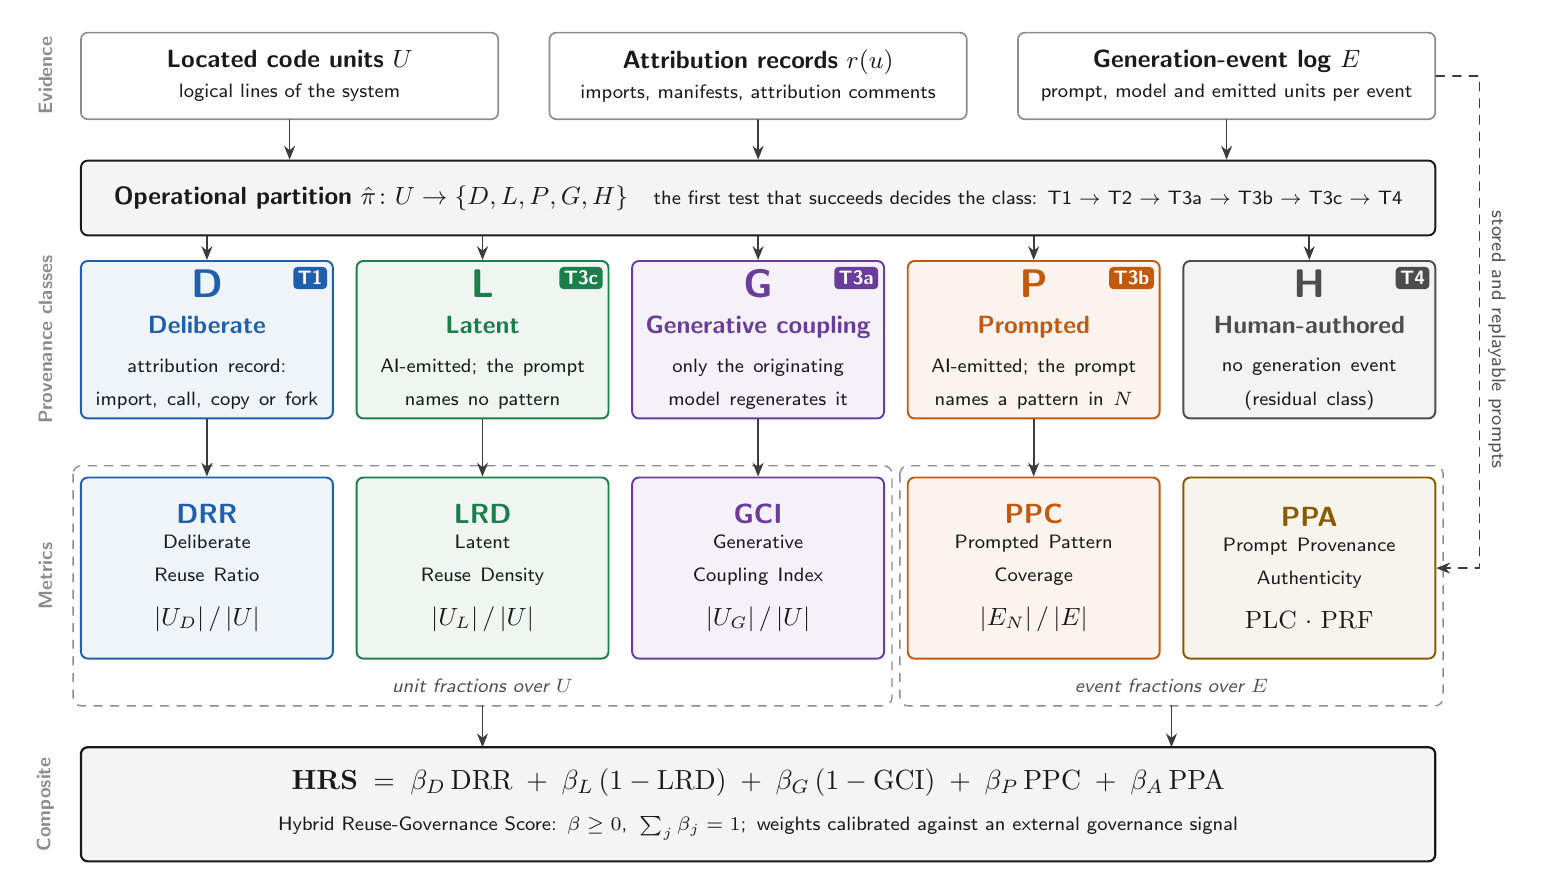
\begin{tikzpicture}[x=1cm,y=1cm]
% ---- column centres (five columns, 3.2 wide, 0.3 gap)
\def\xa{1.6}\def\xb{5.1}\def\xc{8.6}\def\xd{12.1}\def\xe{15.6}
% ---- band labels
\foreach \y/\t in {-0.60/Evidence,-3.95/Provenance classes,-6.95/Metrics,-9.85/Composite}
  \node[rotate=90,font=\scriptsize\bfseries,text=rule] at (-0.45,\y) {\MakeUppercase{\t}};
% ---- evidence
\node[plain,minimum width=5.3cm,minimum height=1.1cm] (U)  at (2.65,-0.6) {\small\textbf{Located code units} $U$\\[-1pt]\scriptsize logical lines of the system};
\node[plain,minimum width=5.3cm,minimum height=1.1cm] (R)  at (8.6,-0.6)  {\small\textbf{Attribution records} $r(u)$\\[-1pt]\scriptsize imports, manifests, attribution comments};
\node[plain,minimum width=5.3cm,minimum height=1.1cm] (E)  at (14.55,-0.6){\small\textbf{Generation-event log} $E$\\[-1pt]\scriptsize prompt, model and emitted units per event};
% ---- protocol bar
\node[draw=ink,line width=0.7pt,rounded corners=2.5pt,fill=ink!5,minimum width=17.2cm,minimum height=0.95cm,align=center] (T) at (8.6,-2.15)
  {\small\textbf{Operational partition} $\hat{\pi}\colon U \to \{D, L, P, G, H\}$\quad\scriptsize the first test that succeeds decides the class:\enspace T1 $\to$ T2 $\to$ T3a $\to$ T3b $\to$ T3c $\to$ T4};
\foreach \n in {U,R,E} \draw[flow] (\n.south) -- (\n.south |- T.north);
% ---- classes
\newcommand{\cls}[6]{% name, x, colour, letter, title, text ; #6 test id drawn separately
  \node[box=#3,minimum width=3.2cm,minimum height=2.0cm,text width=2.9cm] (#1) at (#2,-3.95)
    {{\Large\bfseries\color{#3}#4}\\[1pt]{\small\bfseries\color{#3}#5}\\[2pt]{\scriptsize #6}};}
\cls{D}{\xa}{cD}{D}{Deliberate}{attribution record: import, call, copy or fork}
\cls{L}{\xb}{cL}{L}{Latent}{AI-emitted; the prompt names no pattern}
\cls{G}{\xc}{cG}{G}{Generative coupling}{only the originating model regenerates it}
\cls{P}{\xd}{cP}{P}{Prompted}{AI-emitted; the prompt names a pattern in $N$}
\cls{H}{\xe}{cH}{H}{Human-authored}{no generation event (residual class)}
\foreach \n/\t/\c in {D/T1/cD,L/T3c/cL,G/T3a/cG,P/T3b/cP,H/T4/cH}{
  \draw[flow] (\n.north |- T.south) -- (\n.north);
  \node[font=\scriptsize\bfseries,text=white,fill=\c,rounded corners=1.5pt,inner sep=1.6pt,anchor=north east] at ($(\n.north east)+(-0.08,-0.08)$) {\t};}
% ---- metric group frames
\draw[rule,dashed,line width=0.5pt,rounded corners=3pt] (-0.1,-5.55) rectangle (10.3,-8.6);
\draw[rule,dashed,line width=0.5pt,rounded corners=3pt] (10.4,-5.55) rectangle (17.3,-8.6);
\node[font=\scriptsize\itshape,text=ink!75] at (5.1,-8.35)   {unit fractions over $U$};
\node[font=\scriptsize\itshape,text=ink!75] at (13.85,-8.35) {event fractions over $E$};
% ---- metrics
\newcommand{\met}[6]{% name, x, colour, acronym, long name, formula
  \node[box=#3,minimum width=3.2cm,minimum height=2.3cm,text width=2.95cm] (#1) at (#2,-6.85)
    {{\normalsize\bfseries\color{#3}#4}\\[1pt]{\scriptsize #5}\\[4pt]{\small #6}};}
\met{DRR}{\xa}{cD}{DRR}{Deliberate\\Reuse Ratio}{$|U_D|\,/\,|U|$}
\met{LRD}{\xb}{cL}{LRD}{Latent\\Reuse Density}{$|U_L|\,/\,|U|$}
\met{GCI}{\xc}{cG}{GCI}{Generative\\Coupling Index}{$|U_G|\,/\,|U|$}
\met{PPC}{\xd}{cP}{PPC}{Prompted Pattern\\Coverage}{$|E_N|\,/\,|E|$}
\met{PPA}{\xe}{cA}{PPA}{Prompt Provenance\\Authenticity}{$\mathrm{PLC}\cdot\mathrm{PRF}$}
\draw[flow] (D.south) -- (DRR.north);
\draw[flow] (L.south) -- (LRD.north);
\draw[flow] (G.south) -- (GCI.north);
\draw[flow] (P.south) -- (PPC.north);
% event log audits PPA: routed outside the right edge
\draw[flow,dashed] (E.east) -- ++(0.55,0) |- (PPA.east);
\node[rotate=-90,font=\scriptsize,text=ink!75,anchor=south] at (17.75,-3.95) {stored and replayable prompts};
% ---- composite
\node[draw=ink,line width=0.8pt,rounded corners=2.5pt,fill=ink!5,minimum width=17.2cm,minimum height=1.45cm,align=center] (HRS) at (8.6,-9.85)
  {\normalsize $\mathbf{HRS} \;=\; \beta_D\,\mathrm{DRR} \;+\; \beta_L\,(1-\mathrm{LRD}) \;+\; \beta_G\,(1-\mathrm{GCI}) \;+\; \beta_P\,\mathrm{PPC} \;+\; \beta_A\,\mathrm{PPA}$\\[3pt]
   \scriptsize Hybrid Reuse-Governance Score:\enspace $\beta \ge 0$,\; $\sum_j \beta_j = 1$;\enspace weights calibrated against an external governance signal};
\draw[flow] (5.1,-8.6) -- (5.1,-9.125);
\draw[flow] (13.85,-8.6) -- (13.85,-9.125);
\end{tikzpicture}
\end{document}
